\documentclass[conference]{IEEEtran}
\usepackage{times}

% numbers option provides compact numerical references in the text. 
\usepackage[numbers]{natbib}
\usepackage{multicol}
\usepackage[bookmarks=true]{hyperref}
\usepackage{graphicx,mathrsfs}
\usepackage{float}
\usepackage{subfig,caption}



\pdfinfo{
   /Author (Homer Simpson)
   /Title  (Robots: Our new overlords)
   /CreationDate (D:20101201120000)
   /Subject (Robots)
   /Keywords (Robots;Overlords)
}

\begin{document}

% paper title
\title{Learning Simultaneous Sensory and Motor Representations- (SESEMO)}

% You will get a Paper-ID when submitting a pdf file to the conference system
\author{Berkeley Kids}

%\author{\authorblockN{Michael Shell}
%\authorblockA{School of Electrical and\\Computer Engineering\\
%Georgia Institute of Technology\\
%Atlanta, Georgia 30332--0250\\
%Email: mshell@ece.gatech.edu}
%\and
%\authorblockN{Homer Simpson}
%\authorblockA{Twentieth Century Fox\\
%Springfield, USA\\
%Email: homer@thesimpsons.com}
%\and
%\authorblockN{James Kirk\\ and Montgomery Scott}
%\authorblockA{Starfleet Academy\\
%San Francisco, California 96678-2391\\
%Telephone: (800) 555--1212\\
%Fax: (888) 555--1212}}


% avoiding spaces at the end of the author lines is not a problem with
% conference papers because we don't use \thanks or \IEEEmembership


% for over three affiliations, or if they all won't fit within the width
% of the page, use this alternative format:
% 
%\author{\authorblockN{Michael Shell\authorrefmark{1},
%Homer Simpson\authorrefmark{2},
%James Kirk\authorrefmark{3}, 
%Montgomery Scott\authorrefmark{3} and
%Eldon Tyrell\authorrefmark{4}}
%\authorblockA{\authorrefmark{1}School of Electrical and Computer Engineering\\
%Georgia Institute of Technology,
%Atlanta, Georgia 30332--0250\\ Email: mshell@ece.gatech.edu}
%\authorblockA{\authorrefmark{2}Twentieth Century Fox, Springfield, USA\\
%Email: homer@thesimpsons.com}
%\authorblockA{\authorrefmark{3}Starfleet Academy, San Francisco, California 96678-2391\\
%Telephone: (800) 555--1212, Fax: (888) 555--1212}
%\authorblockA{\authorrefmark{4}Tyrell Inc., 123 Replicant Street, Los Angeles, California 90210--4321}}


\maketitle

%\begin{abstract}
%\end{abstract}

\IEEEpeerreviewmaketitle

Redundancy reduction \cite{barlow1961possible}, edge detection \cite{hubel1968receptive}  and hierarchical representations \cite{krizhevsky2012imagenet} have been the main stay for lot of work in computer vision and vision neuroscience to represent sensory data. But, these representations do not directly lend themselves to action. It has been hypothesized \cite{o2001sensorimotor} that brain probably represents sensory information in a way that helps an organism to act in the world.  

Philipona and O'Regan \cite{philipona2003there,philipona2003perception} showed that the joint manifold of sensory and action space taken together has a lower dimensionality than that obtained by simply adding the dimensions of motor and sensory spaces. An observation which explains this is that motion of an object in the world and the equal but opposite motion of the organism with the object being stationary leads to the same sensory percept. It`s the relative motion which matters. In other words, sensory and motor spaces are `compensable'. This insight is probably employed by organisms to achieve stability of percept. For example, even when we humans are moving we perceive the world to be stationary. 


In this work we consider the problem of joint learning of sensory and motor representations within the context of percept stabilization.  This goal is interesting because it lets the agent to build a sensory representation that is coupled with its actions. We assume that agent has no apriori knowledge of its kinematic model nor does it have any meaningful representations of its sensory stimulus, i.e. the agent is in the state of `tabula rasa' initially.  


In overactuated motor systems (high degrees of freedom/redundancy) training a control model becomes challenging. \cite{rolf2012efficient} explored learning of inverse kinematics to reach a certain goal state. Other works have proposed solutions based on the concepts of motor primitives \cite{schaal2005learning}. However, no work has looked at learning such primitives from the statistics of the motion that an agent needs to perform to achieve a goal.  Here, we wish to explore the idea of learning motor primitives that can then be composed sequentially to perform actions. 
Such a representation regularizes the space of possible motor actions and allows the agent to conduct high level planning of actions by providing it with a vocabulary of primitive motions to chose from. That is to say, at each time step we no longer have to specify the control sequence for each controller but the problem is now of choosing an appropriate motion primitive (aka basis element). This is also a biologically plausible system, especially considering the fact that spinal reflexes (akin to motion primitives) and cortical motor systems (high level planning)  work closely to make complex motions possible\cite{kandel2000principles}. 

It seems likely that for a robotic agent, a hierarchical control system with some low-level task dependent reflex circuits that are modulated by high level commands will lead to easier planning. Work of \cite{todorov2004optimality} in optimal control theory literature also talks of related ideas. 

The main ideas proposed in this work can be summarized as following: 
\begin{itemize}
\item Learning of a motor basis for control (just like gabor functions form a basis for image patches.) 
\item Goal dependent joint estimation of sensory and motor representations.
\item Developing adaptive fault-tolerant sensorimotor representations. 
\end{itemize}


\section{Model}
\begin{figure}[t!]
\centering
\subfloat{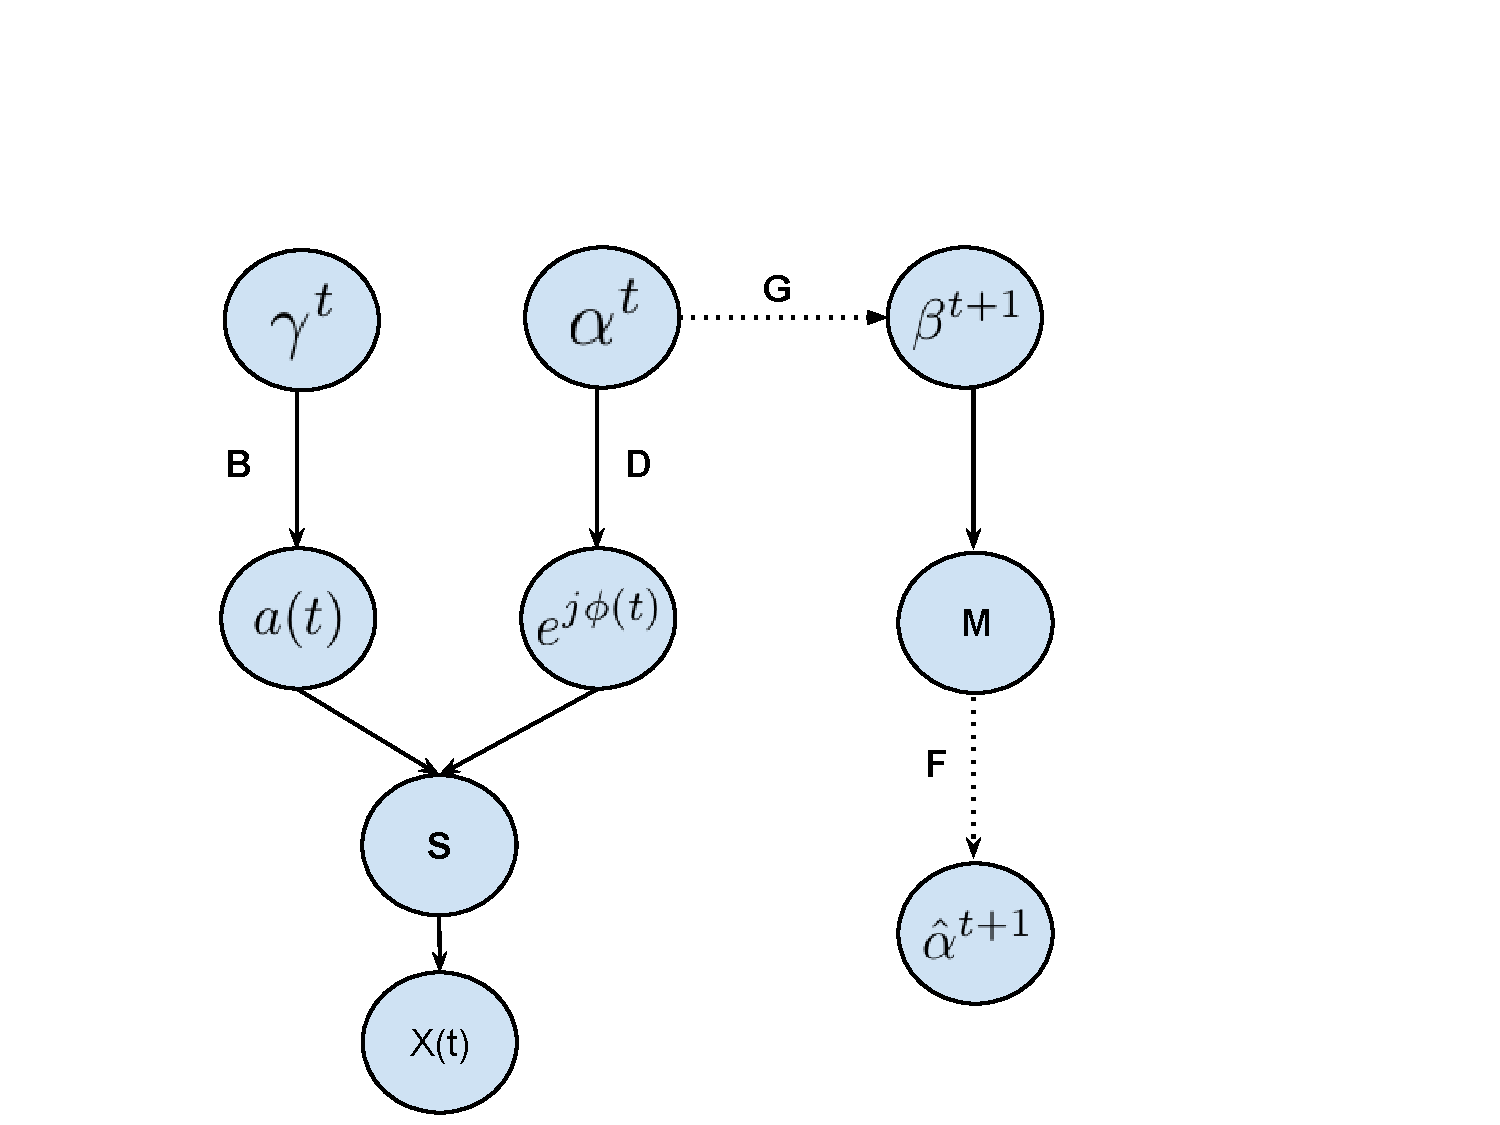
\includegraphics[width=0.75\linewidth]{sesemo1.pdf} } 
\caption{This figure depicts a graphical model representation of the sensory-motor system of the agent. Please refer to the text for more details. Note, the term graphical model is used in a loose sense.}
\label{fig:sesemo}
\end{figure}

Fig \ref{fig:sesemo} depicts the sensory-motor system of the agent. \textbf{X(t)} is the sequence of images (frames) that fall on the retina (say). We then learn a sparse generative sensory representation along the lines of Cadieu \& Olshausen  \cite{cadieu2012learning} that tries to account for both form ($\gamma^{t})$  and motion$(\alpha^{t})$ separately using complex basis elements. We refer the reader to \cite{cadieu2012learning} for more details for its training.

$\mathcal{G}$ transforms the motion component of the sensory percept to the motor primitive space $\beta^{t+1}$ and the input to the actuators is given by $M\beta^{t+1}$.
\begin{eqnarray}
\beta^{t+1} = \mathcal{G} \alpha^{t}
\end{eqnarray}
In order to stabilize the percept, at every time step the agent must move in a way which would compensate for the change in visual stimulus caused due to motion of objects in the environment. Consequently, at every time step, the agent tries to predict the sensory percept which it expects to see at the next time step(i.e. $\hat{\alpha}^{t+1}$). Note, in contrast to predicting the next image frame in the pixel space, the agent predicts in the parameter space - i.e the agent predicts the sensory percept it would infer at the next time step instead of the pixel values themselves. This prediction is expressed as following:
\begin{eqnarray}
\hat{\alpha}^{t+1} = \sum_{i=t-T+1}^{t-1}  H_{t-i} \alpha(t-i) + \mathcal{F}\mathcal{M}\beta^{t+1} 
\end{eqnarray}
where, $\mathcal{F}$ is the transformation from the motor space to sensory parameter space and $H_{t-i}$ is the effect of the sensory parameters inferred at time t-i on the prediction of time point t+1, and T is the number of past time steps used to make such a prediction. 

In order to learn the sensorimotor representation the agent optimizes the following:
\begin{eqnarray}
\min_{F,M,G,\tau} \| \alpha^{t+1} - \hat{\alpha^{t+1}} \|_{2} \\
\nonumber \textit{s.t.} \hspace{3mm} \forall i \sum_{j}  |G_{ij}| = c_1  \hspace{2mm}, \forall k \sum_{l}  |\mathcal{F}_{kl}| = c_2 
\end{eqnarray}

which forces the agent's prediction $(\hat{\alpha^{t+1}})$ to be close to the observed percept$({\alpha^{t+1}})$. Further, we constrain the row sums of $G$ and $\mathcal{F}$ to learn sparse $G$, $\mathcal{F}$ respectively. These matrices being sparse in turn enforces that $\beta,\hat{\alpha} $ are also sparse.

\section{Discussion}
Perceptual stabilization is a problem that many if not most animals have solved. In birds, eye movements are replaced with compensatory head movements. In this work, we wish to explore a framework that learns in sensorimotor loops. There is paucity of models that try to describe learning in these two seemingly disparate domains. 

While the model is nascent, thinking of learning sensory and motor representations simultaneously can be a way to model the statistics of the world and exploring the control space efficiently. Future models can hope to explore ideas from hierarchical control to explore longer trajectory primitives to be learnt. An important consideration for such problems is to explore the temporal nature of feedback between the two systems. The sampling rate of the sensory and motor system might vary drastically between agents.


\section{ Acknowledgments} 

Discussions with Jitendra Malik and Tony Bell motivated a lot of this work as well. Special thanks to Pavan Ramkumar, Northwestern University for helping clarify a lot of ideas through discussions. Special thanks to Bruno Olshausen for urging us to think about sensorimotor representations. We would also like to thank our respective funding agencies - Fulbright Scholar Program. NGA. NIH. UC Berkeley.

All the preliminary code for this project can be found on our github\footnote{github.com/rctn/sesemo} link.


\bibliography{cs287_final}
\bibliographystyle{plainnat}

\end{document}


